\documentclass[11pt]{article}

\usepackage[margin=1in]{geometry}
\usepackage{amsmath}
\usepackage{amssymb}
\usepackage{booktabs}
\usepackage{graphicx}
\usepackage{natbib}
\setlength{\bibsep}{1.0pt}
\usepackage[hidelinks]{hyperref}
\usepackage{xcolor}
\usepackage{placeins}
\usepackage[protrusion=true,expansion=false]{microtype}

\title{TOI-3492.01: A Persistent Transit-like Signal in Six TESS Sectors}

\author{Furkan \c{S}en\\[4pt]
  \small Department of Astronomy and Space Sciences, Ankara University}

\date{23 July 2026}

% -----------------------------------------------------------------------
\begin{document}
% -----------------------------------------------------------------------

\maketitle

\begin{abstract}
TOI-3492.01 (TIC~81077799) is a TESS Object of Interest with an official
period of $P=9.2224171$~d.  We analyze six publicly available 120-s SPOC
light curves spanning five years.  A several-thousand-ppm transit-like signal
is present at the official ephemeris in every sector, although formal
sector-depth estimates are heterogeneous.  A circular fit to phase-folded,
8-minute-binned photometry is retained only as a descriptive reference model;
window and cadence-mask tests show that its statistical intervals do not
capture the full reduction and baseline sensitivity.  If the event is
planetary, originates on TIC~81077799, and the catalog single-star parameters
are correct, the reference radius ratio corresponds to a giant-planet-sized
companion.  Native-cadence 120-s and 20-s fits are not reported as measurements
because their convergence and noise-model gates fail.  Odd/even and fixed
phase-0.5 secondary checks are inconclusive screening tests, and archival SPOC,
Gaia, aperture, and first-pass difference-image diagnostics do not provide
calibrated source localization.  No formal false-positive probability,
eccentricity, mass, statistical validation, or dynamical confirmation is
claimed.  TOI-3492.01 remains an unvalidated and unconfirmed transit-like
candidate requiring PRF-level localization, high-resolution imaging,
spectroscopy, and epoch radial velocities.
\end{abstract}

% -----------------------------------------------------------------------
\clearpage
\section{Introduction}
% -----------------------------------------------------------------------

The Transiting Exoplanet Survey Satellite (TESS; \citealt{Ricker2015}) has
identified thousands of transiting planet candidates around bright,
nearby stars.  Among the most astrophysically informative subsets are
short-period giant candidates around evolved hosts.  All else being equal, as
a star departs the main sequence and expands, transit probability and duration increase
while the fractional depth of a fixed-radius companion decreases
\citep{Seager2003}.  Tidal interactions and increased irradiation can reshape
the system architecture \citep{Grunblatt2022,Grunblatt2023,Saunders2024}.
Systematic characterization of such candidates therefore constrains
theories of hot-Jupiter formation and orbital migration around intermediate-
and high-mass stars.  Recent TESS studies of planets around subgiants and
evolved hosts show that short-period giants in this regime are sparse and
valuable tracers of tidal evolution, eccentricity excitation, and spin-orbit
realignment \citep{Grunblatt2022,Grunblatt2023,Chontos2024,Saunders2024}.  The
confirmed system TOI-1842b, a warm Saturn at a similar period around an
evolving subgiant, provides a useful comparison point for TOI-3492.01 while
also illustrating the level of follow-up required for confirmation
\citep{Wittenmyer2022}.

TOI-3492.01 is a TESS Object of Interest associated with TIC~81077799.
No prior photometric characterization of this candidate has been published
in the refereed literature or on arXiv at the time of writing.
The official TOI ephemeris gives $P = 9.2224171$~d and a transit depth of
approximately 3110~ppm.  Stellar parameters from TIC~v8 \citep{Stassun2019}
indicate a large, low-density evolved F-type host ($R_\star \approx 2.6\,R_\odot$,
$\log g \approx 3.71$) rather than a solar-radius dwarf, making the candidate's
physical radius substantially larger than a naive main-sequence assumption
would imply.  This work presents an independent photometric
characterization of TOI-3492.01 using the 120~s cadence SPOC light curves.
A set of photometric, catalog, and archival false-positive diagnostics is
reported without converting them into an unsupported validation probability.

This is a photometry-only characterization.  There is no radial-velocity
mass measurement or high-resolution imaging.  Independent ground-based
spectroscopic stellar parameters are also unavailable; the principal
limitations are discussed in Section~\ref{sec:discussion}.
TOI-3492.01 is therefore reported as a transit-like candidate; no statistical
validation or dynamical confirmation is claimed.

% -----------------------------------------------------------------------
\section{Observations and Data Reduction}
% -----------------------------------------------------------------------

Public TESS SPOC light curves \citep{Jenkins2016} were retrieved from the
Mikulski Archive for Space Telescopes (MAST) with \texttt{lightkurve}
\citep{Lightkurve2018}.  TIC~81077799 has nine SPOC products in the local
search inventory: 120~s products in Sectors~37, 63, 64, 90, 99, and~100,
plus additional 20~s products in Sectors~90, 99, and~100.  The corrected
analysis uses only the six 120~s products.  This avoids duplicate weighting
of sectors with both 20~s and 120~s products.

The corrected reference light curve contains
102\,502 finite 120~s measurements.  Each sector was normalized
independently using out-of-transit flux near the official ephemeris.  Strong
positive outliers were removed while preserving transit-like negative
excursions.  No transit-suppressing flattening was applied near the expected
transit windows.

The adopted PDCSAP products already include SPOC systematics and crowding
corrections.  This work then applies per-sector constant normalization and
asymmetric outlier rejection; it does not apply an additional flattening or
polynomial detrending operation.
The resulting phase-folded reference light curve is shown in
Figure~\ref{fig:fold}.

\begin{figure}[ht]
\centering
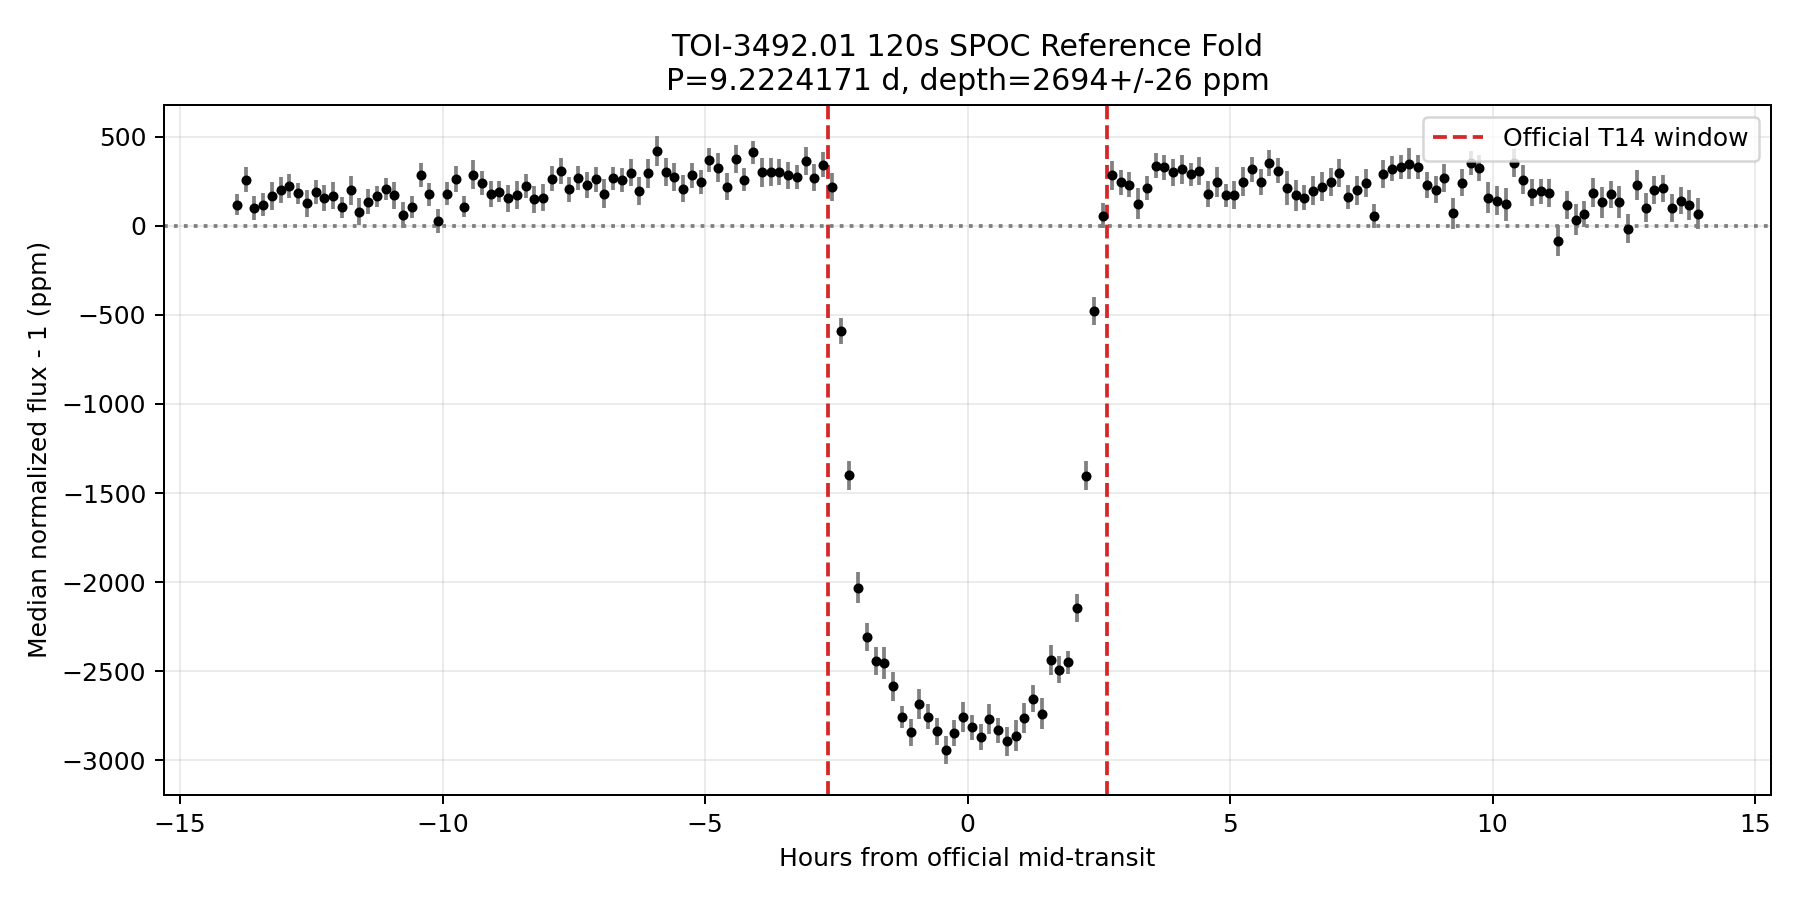
\includegraphics[width=0.95\linewidth]{figures/toi3492_120s_reference_fold.png}
\caption{Corrected 120~s SPOC reference light curve folded on the official
  ephemeris ($P=9.2224171$~d, $T_0=2314.521155$~BTJD, where
  $\mathrm{BTJD}=\mathrm{BJD}_{\rm TDB}-2457000$).  Each of the six
  sectors was normalized independently before folding; no transit-suppressing
  flattening was applied.  Red dashed lines mark the official transit-duration
  window.  This product supports the descriptive phase-folded reference fit.}
\label{fig:fold}
\end{figure}

% -----------------------------------------------------------------------
\section{Stellar Characterization}
\label{sec:stellar}
% -----------------------------------------------------------------------

Stellar parameters were obtained from TIC~v8 \citep{Stassun2019} via
\texttt{astroquery}.  The catalog parameters used for conditional scale
estimates are listed in
Table~\ref{tab:stellar}.  The combination of low surface gravity
($\log g \approx 3.71$), large radius ($R_\star \approx 2.6\,R_\odot$),
and low mean density ($\rho_\star \approx 0.072\,\rho_\odot$) is
physically inconsistent with a main-sequence dwarf and is characteristic
of an evolved subgiant-like host, despite the TIC \texttt{lumclass=DWARF}
classification.

\begin{table}[ht]
\centering
\caption{Catalog stellar parameters used for conditional scale estimates for
  TIC~81077799.  TIC~v8 supplies the
  catalog values; the mean density is derived from the listed mass and radius,
  its uncertainty is calculated using first-order propagation of independent
  errors, and the
  metallicity is an explicit limb-darkening interpolation assumption.}
\label{tab:stellar}
\begin{tabular}{lc}
\toprule
Parameter & Value \\
\midrule
Effective temperature, $T_{\rm eff}$ & $6332 \pm 134$ K \\
$\log g$ (cgs)   & $3.7075 \pm 0.0835$ \\
Stellar radius, $R_\star$          & $2.5926 \pm 0.1094\,R_\odot$ \\
Stellar mass, $M_\star$            & $1.25 \pm 0.19\,M_\odot$ \\
Derived mean density, $\rho_\star$ & $0.0717 \pm 0.0140\,\rho_\odot$ \\
Assumed metallicity, $[\mathrm{Fe}/\mathrm{H}]$ & $0.0 \pm 0.15$ dex \\
TESS magnitude, $T_{\rm mag}$ & 8.450 \\
Distance         & $201.96 \pm 1.27$ pc \\
\bottomrule
\end{tabular}
\end{table}

The listed mass and radius imply $\rho_\star \approx 0.072\,\rho_\odot$ and a
luminosity of approximately $9.7\,L_\odot$, further supporting the evolved subgiant-like
nature of the host. This evolved-host interpretation is central to the physical scale of the
candidate: the same radius ratio implies a much larger companion around a $2.6\,R_\odot$
star than around a main-sequence solar-radius star.

As an external catalog-model cross-check, Gaia~DR3 GSP-Phot/FLAME gives
$R_\star=2.671\,R_\odot$, $M_\star=1.514\,M_\odot$, and
$L_\star=8.68\,L_\odot$ at the catalog medians.  These imply
$\rho_\star=0.0794\,\rho_\odot$, a Keplerian
$a/R_\star=7.96$ for negligible companion mass, and $R_p=15.94\,R_\oplus$
when combined with the diagnostic reference
radius ratio.  Thus a second catalog model family also supports an evolved
host.  Gaia's narrow
quoted percentile intervals are internal model intervals and are not treated
as complete external uncertainties.  A conflicting Gaia GSP-Spec solution
has a non-clean flag string and is retained only in the machine-readable
provenance, not adopted.

As a further scale check, we retrieved and froze a set of 2MASS and AllWISE
photometric measurements selected using the catalog quality flags, then fitted a reddened
blackbody with a 0.05-mag common
model/passband error floor and a TIC/Gaia temperature-mixture prior.  This
gives $R_\star=2.509^{+0.055}_{-0.050}\,R_\odot$ and
$L_\star=9.79^{+0.60}_{-0.60}\,L_\odot$.  The chain satisfies the
$50\tau$ heuristic, but monochromatic blackbody photometry is not a substitute
for passband-integrated atmosphere and isochrone models.  We therefore use
this only as an approximate SED radius cross-check and retain the broader TIC
uncertainties for conditional physical-scale scenarios.  An equal-brightness unresolved
binary branch would reduce each component's SED radius by $\sqrt{2}$; without
binary isochrones it provides no defensible component mass, density, or age.

Quadratic limb-darkening coefficients in the TESS band were fixed to
$u_1 = 0.393$, $u_2 = 0.150$, computed using \texttt{LDTk}
\citep{Parviainen2015} with the PHOENIX specific-intensity library
\citep{Husser2013} at the adopted $T_{\rm eff}$, $\log g$, and
$[\mathrm{Fe}/\mathrm{H}]$.  TIC~v8 has no metallicity value for this target,
so the interpolation assumes $[\mathrm{Fe}/\mathrm{H}]=0.0\pm0.15$~dex; this
is an atmosphere-grid input width, not a metallicity measurement.
The reference quadratic law is
$I(\mu)/I(1)=1-u_1(1-\mu)-u_2(1-\mu)^2$, where $I(\mu)$ is the emergent
specific intensity and $\mu$ is the cosine of the angle between the local
surface normal and the line of sight.
This atmosphere-model prediction replaces the previous approximate fallback formula
($u_1 \approx 0.406$, $u_2 \approx 0.157$).

Four ground-based spectroscopic archives were searched: APOGEE~DR17,
LAMOST~DR10, GALAH~DR3, and RAVE~DR6.  The search targeted independent
$T_{\rm eff}$ and $\log g$ measurements of TIC~81077799.  Automated
5-arcsec cone searches returned zero matches across all four catalogs.  The
non-detection by LAMOST is expected given the
star's southern declination ($\delta = -53.7^\circ$), but the absence from
APOGEE, GALAH, and RAVE means that no independent ground-based spectroscopic
$T_{\rm eff}$, $\log g$, or $[\mathrm{Fe}/\mathrm{H}]$ measurement is available
from these archives.
Gaia~DR3 reports a mean RVS velocity of $13.33\pm0.21$~km~s$^{-1}$ from
13 field-of-view visits spanning 864~d, with a robust-amplitude statistic of
2.08~km~s$^{-1}$ and a velocity-constancy $p$-value of 0.046; the robust
amplitude is a catalog variability statistic, not an orbital range or
semi-amplitude.  Epoch
velocities are not public, so these summary values cannot provide an orbit
or companion mass; they motivate dedicated RV monitoring.  The stellar parameters
used below are therefore photometric/catalog values: TIC~v8 (broadband SED
fitting plus Gaia parallax; \citealt{Stassun2019}) and Gaia GSP-Phot (BP/RP
spectrophotometry).  TIC~v8 values are used only for explicitly conditional
scale calculations in this work.  This lack of independent spectroscopic atmospheric parameters
means that the $a/R_\star$ tension discussed below cannot be resolved with
existing public data; resolving it would require new dedicated spectroscopy.

% -----------------------------------------------------------------------
\section{Orbital Ephemeris}
% -----------------------------------------------------------------------

The official TOI ephemeris is $P = 9.2224171$~d and
$T_0 = 2314.521155$~BTJD \citep{NASAExoplanetArchiveTOI}.  A Box
Least-Squares (BLS; \citealt{Kovacs2002}) period search on the 120~s SPOC
products recovers a periodic signal near 9.222~d in all tested modes.
Because this is a targeted recovery using the known candidate, it demonstrates
pipeline consistency rather than independently confirming the quoted period
and epoch precision.

\begin{table}[ht]
\centering
\caption{Ephemeris and 120~s period-search diagnostics.}
\label{tab:ephemeris}
\begin{tabular}{lc}
\toprule
Quantity & Value \\
\midrule
Official period             & $9.2224171 \pm 0.0000098$~d \\
Official $T_0$              & $2314.521155 \pm 0.000615$~BTJD \\
120~s BLS grid maximum      & 9.222~d (0.0019-d grid spacing) \\
Robust 120~s depth at official ephemeris & $2694 \pm 26$~ppm \\
Official TOI depth          & $3109.8 \pm 36.9$~ppm \\
\bottomrule
\end{tabular}
\end{table}

The robust depth in Table~\ref{tab:ephemeris} is a fixed-window diagnostic
based on in-transit and out-of-transit data.  The transit model described in
Section~\ref{sec:model} is also diagnostic and is not an adopted native-cadence
posterior.

% -----------------------------------------------------------------------
\section{Descriptive Transit Reference and Sensitivity Analysis}
\label{sec:model}
% -----------------------------------------------------------------------

For descriptive comparison with the official TOI solution, the corrected
120~s light curve was phase-folded on the official ephemeris,
selected over $|t-T_c|<13$~h (a 13-h half-width and 26-h total window),
median-binned to 8-minute intervals, and fitted
with an analytic transit model using \texttt{batman}
\citep{Kreidberg2015}.  The fitted parameters were $R_p/R_\star$,
$a/R_\star$, impact parameter $b$, a baseline term, and a log-uniform
white-noise floor.  The orbital period
and reference epoch were fixed to the official TOI values.  Eccentricity
was fixed to $e=0$ in the working model — not because circularity is proven,
but because transit photometry alone does not robustly constrain eccentricity
for this target.  Limb darkening was fixed to the reference TESS-band
coefficients.  The model was integrated over each 8-minute inference bin.
The likelihood used the robust standard error of each bin plus a fitted
log-uniform white-noise floor.  Hard bounds were
$0.025<R_p/R_\star<0.09$, $4<a/R_\star<13$,
$0\leq b<1+R_p/R_\star$, $0.995<c<1.005$, and 10--2000~ppm for the
white-noise floor, where $c$ is the multiplicative baseline.  Here $t$ is the
observation time and $T_c$ is the transit-center time predicted by the fixed
ephemeris.  No stellar-density prior was applied.

MCMC sampling was performed with \texttt{emcee} \citep{ForemanMackey2013} using 48
walkers, 1200 burn-in steps, and 6000 production steps.  After discarding the
first 750 production steps, the flat posterior comprises 252\,000 samples
over five parameters.  Estimated integrated autocorrelation times are
55.4--90.3 production steps, and the production run spans at least 66
autocorrelation times for every fitted parameter,
satisfying the conservative $50\tau$ reporting heuristic.
The symmetric uncertainties quoted for the fitted transit parameters use the
larger of the distances from the posterior median to the 16th and 84th
percentiles; they are not posterior standard deviations.

The circular photometry-only fit is retained only as a descriptive reference.
It is not used to claim a stellar-density discrepancy or eccentricity because
the accepted window/mask family, correlated-noise stationarity, reduction-family
propagation, stellar posterior, and native-cadence convergence requirements are
not all satisfied.  Exploratory density-informed eccentric fits are therefore
not reported as scientific measurements or model-selection evidence.

As deterministic sensitivity checks, the maximum-likelihood fit was repeated
for 4-, 8-, and 12-minute bins and for window half-widths of 10, 13, and
16 hours.  At the 13-hour reference half-width, changing bin size shifted $R_p/R_\star$ by at
most 0.2 reported posterior half-widths and $a/R_\star$ by at most 0.2
reported posterior half-widths.  Across all nine variants, the largest shifts
were approximately 1.2 reported posterior half-widths in $R_p/R_\star$ and
0.5 in $a/R_\star$, occurring for the shortest fit window.  These
optimization checks illustrate sensitivity around the reference scale but do not replace full
posterior reruns with a correlated-noise model.

Because ``13-hour window'' can alternatively mean a 13-h total width, we also
performed a separate full MCMC fit over $|t-T_c|<6.5$~h, keeping the likelihood,
priors, 8-minute bins, exposure integration, sampler settings, and seed fixed.
Its 6000-step production chain spans 80--99 estimated autocorrelation times and
gives $R_p/R_\star=0.05567^{+0.00039}_{-0.00040}$,
$a/R_\star=10.17^{+0.32}_{-0.29}$, and $b=0.730^{+0.019}_{-0.021}$.  Relative
to the 26-h reference window, the radius ratio shifts by 1.95
reference-posterior half-widths and $a/R_\star$ by 0.96.  The shift
demonstrates that the reference statistical intervals do not include
fit-window choice.  Neither window is adopted as a final native-cadence
solution.

We also performed a separate native-cadence robustness analysis without
changing the descriptive reference fit.  It retained all 12\,051 120~s points
within $|t-T_c|<13$~h and integrated the model over the
actual 120~s
exposures.  Geometry was shared, while each sector had an independent radius
ratio and jitter; sector linear baselines were profiled analytically.  Period
and epoch were sampled with the official uncertainties, and limb darkening was
sampled in the physical $q_1,q_2$ parameterization with a 0.05 external floor
on each $u$ coefficient.  The transformation is
$q_1=(u_1+u_2)^2$ and $q_2=u_1/[2(u_1+u_2)]$.  Fixed out-of-transit AR(1) coefficients of
0.00--0.27 supplied a short-timescale pre-whitening sensitivity test.  The
same model was applied separately to native 20~s points in Sectors~90, 99,
and~100.  The two same-pixel cadence products are correlated diagnostics, not
independent evidence.  The
120~s and 20~s production chains span only 8.6--12.1 and 9.4--10.9
estimated autocorrelation times, respectively, rather than the conservative
$50\tau$ target.  Their parameter intervals are omitted because they are not
adopted posteriors.  The model does not include event-level timing offsets, an
alternative atmosphere prescription for limb darkening, a hierarchical
sector-depth excess-scatter term, or marginalized AR(1) and baseline
uncertainties.  Sector radius ratios are independent nuisance parameters and
their reported mean is an arithmetic diagnostic, not a hierarchical common
radius.  These omissions prevent adoption of a native-cadence geometry.
Figures~\ref{fig:fit} and \ref{fig:corner} show the descriptive reference fit and
the corresponding posterior distributions, respectively.

\begin{figure}[ht]
\centering
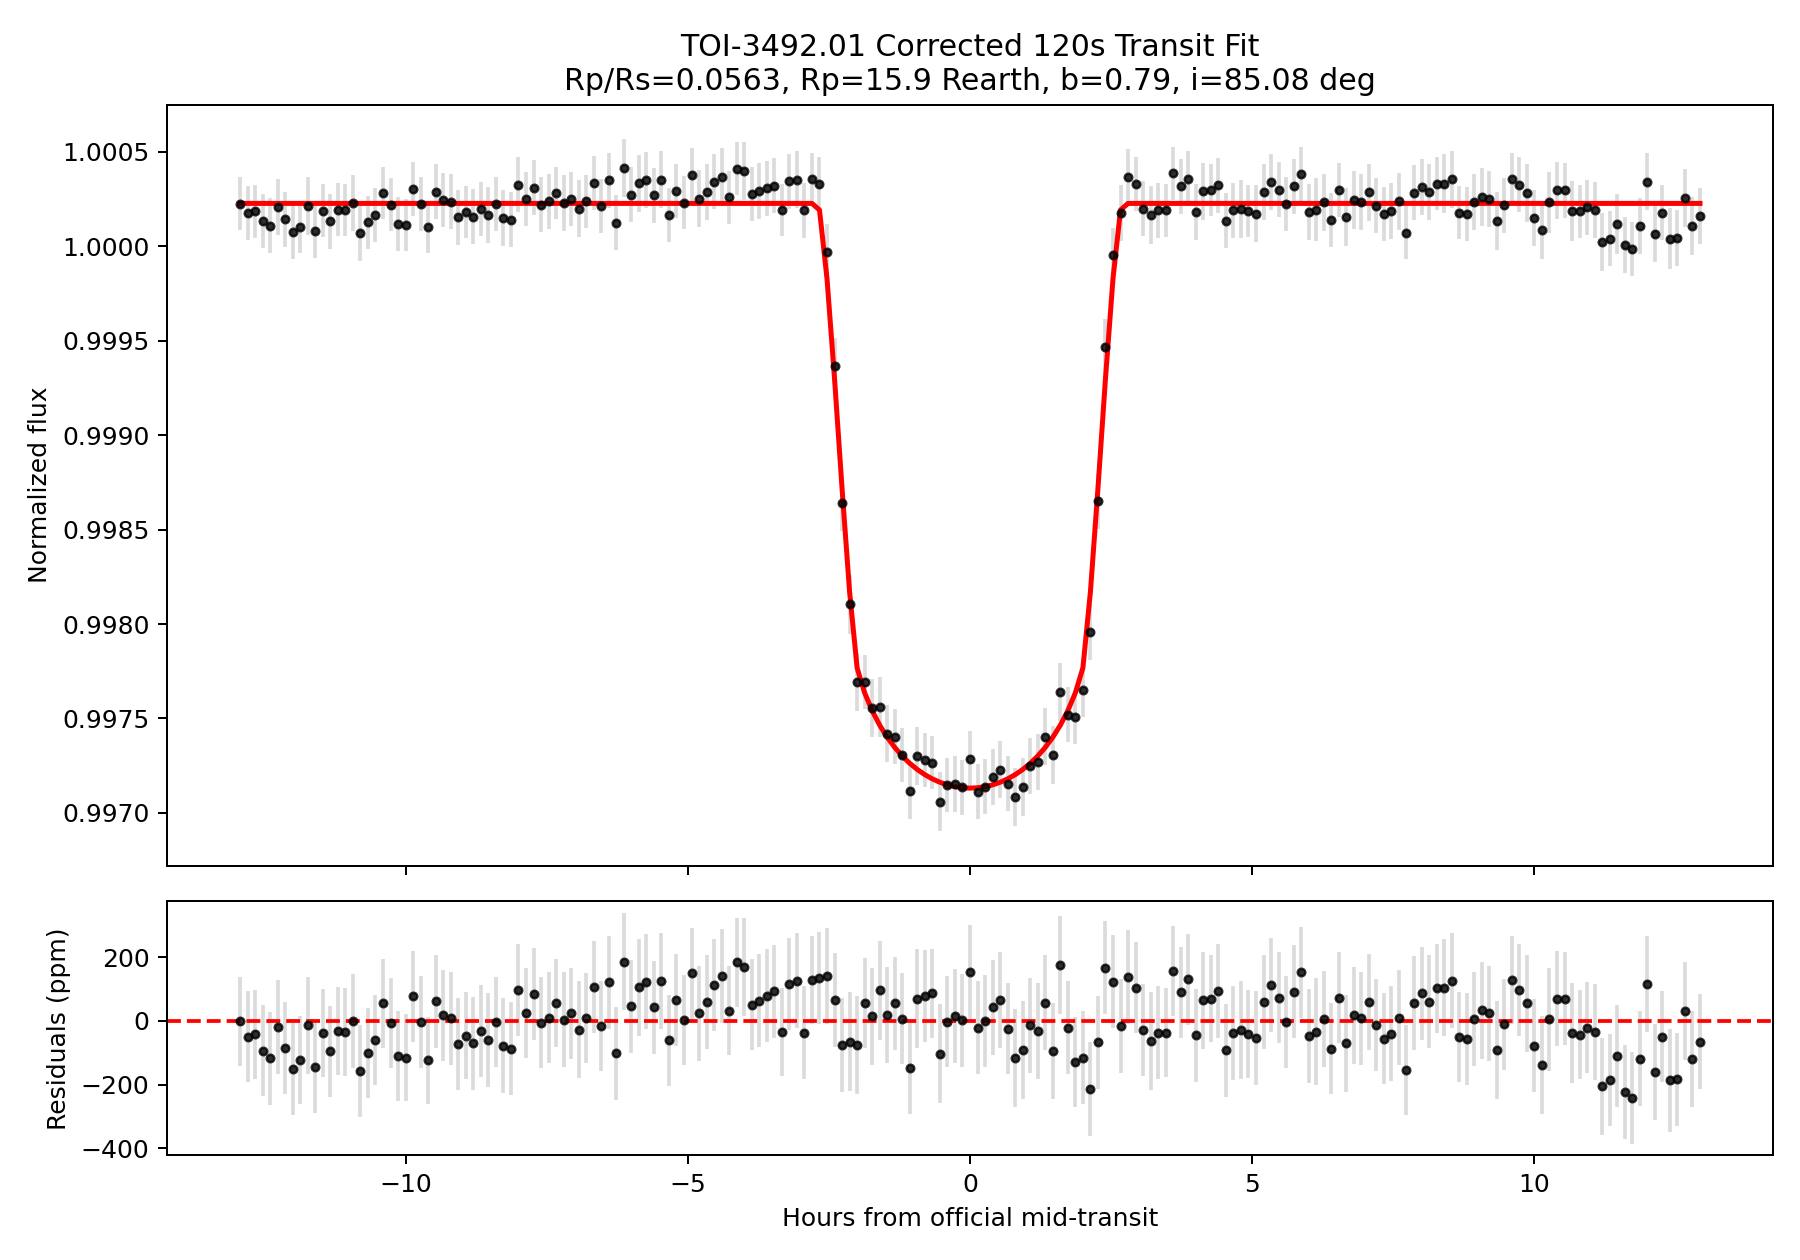
\includegraphics[width=0.95\linewidth]{figures/toi3492_transit_fit_120s_corrected.png}
\caption{Corrected 120~s phase-folded transit fit for TOI-3492.01.
  The model uses the official ephemeris, a circular orbit ($e=0$ fixed),
  quadratic limb-darkening coefficients from \texttt{LDTk}
  \citep{Parviainen2015,Husser2013} ($u_1=0.393$, $u_2=0.150$), and the corrected 120~s
  reference light curve.  The black curve is the best-fit diagnostic
  \texttt{batman} model; gray points are binned photometry.  Residuals are
  shown in the lower panel.}
\label{fig:fit}
\end{figure}

\begin{figure}[ht]
\centering
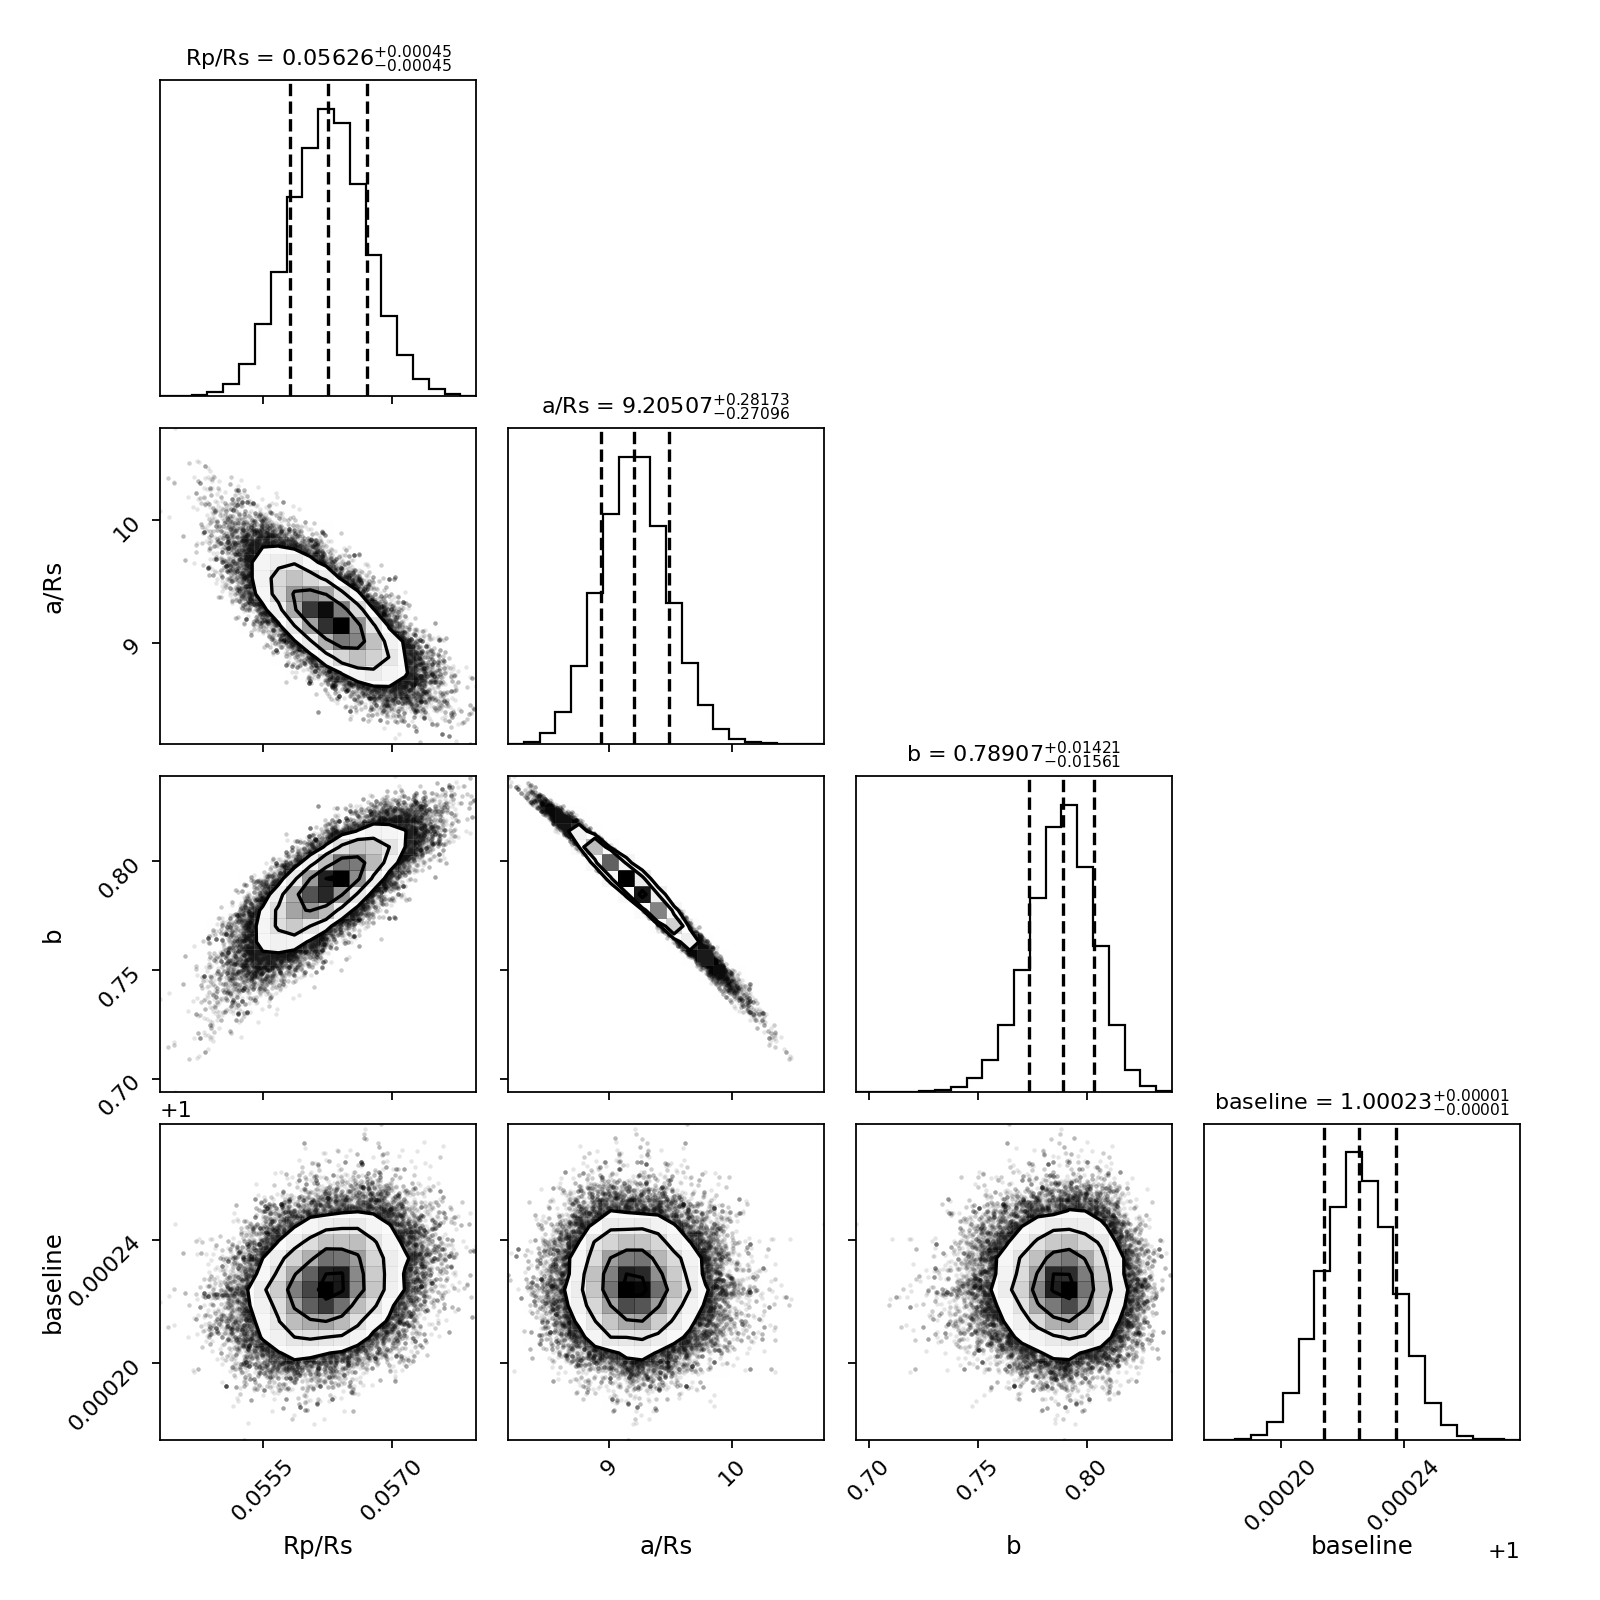
\includegraphics[width=0.80\linewidth]{figures/toi3492_corner_120s_corrected.png}
\caption{Posterior distributions for the five free parameters of the
  corrected 120~s circular transit fit: $R_p/R_\star$, $a/R_\star$,
  impact parameter $b$, the baseline term, and the fitted noise floor.
  The MCMC run used 48 walkers and 6000 production steps, with a mean
  acceptance fraction of 0.512.}
\label{fig:corner}
\end{figure}

% -----------------------------------------------------------------------
\section{Results}
% -----------------------------------------------------------------------

The descriptive reference parameters and conditional scale estimates are summarized
in Table~\ref{tab:planet}.

\begin{table}[ht]
\centering
\caption{Diagnostic phase-folded transit parameters and conditional scenario
  properties for TOI-3492.01.  These are not adopted native-cadence results.}
\label{tab:planet}
\renewcommand{\arraystretch}{1.16}
\begin{tabular}{lc}
\toprule
Parameter & Value \\
\midrule
\multicolumn{2}{l}{\textit{Diagnostic fitted transit parameters}} \\[2pt]
Period, $P$                 & $9.2224171$~d (fixed to official TOI) \\
Reference epoch, $T_0$      & $2314.521155$~BTJD (fixed) \\
$R_p/R_\star$               & $0.05472 \pm 0.00049$ \\
$a/R_\star$                 & $10.60 \pm 0.45$ \\
Impact parameter, $b$       & $0.705 \pm 0.032$ \\
Eccentricity                & $0$ (fixed) \\
Inclination (derived)       & $86.19 \pm 0.32^\circ$ \\[4pt]
\multicolumn{2}{l}{\textit{Quantities derived from the transit profile}} \\[2pt]
Mid-transit model depth     & $\approx3094\,\mathrm{ppm}$ (at the marginal posterior medians) \\
Area ratio, $(R_p/R_\star)^2$ & $2994^{+51}_{-53}\,\mathrm{ppm}$ \\
Transit duration, $T_{14}$  & $5.233^{+0.041}_{-0.042}\,\mathrm{h}$ \\[6pt]
\multicolumn{2}{l}{\textit{Catalog-conditional derived quantities}} \\[2pt]
Candidate radius, $R_p\,(R_\oplus)$ & $15.47 \pm 0.66$ \\
Candidate radius, $R_p\,(R_{\rm J})$ & $1.38 \pm 0.06$ \\
Semimajor axis, $a$         & $0.0927^{+0.0044}_{-0.0049}$~AU \\
Stellar luminosity          & $9.72^{+1.21}_{-1.10}\,L_\odot$ \\
Incident flux, $S$          & $1135^{+193}_{-161}\,S_\oplus$ \\
Equilibrium temperature, $T_{\rm eq}$ & $1616^{+65}_{-61}\,\mathrm{K}$ \\[6pt]
\multicolumn{2}{l}{\textit{MCMC diagnostics}} \\[2pt]
Walkers                     & 48 \\
Burn-in / production steps  & 1200 / 6000 \\
Flat samples                & 252\,000 \\
Mean acceptance fraction    & 0.512 \\
Autocorrelation time $\tau$ & 55.4--90.3 steps \\
Production length / $\tau$  & 66.4--108.4 \\
\bottomrule
\end{tabular}
\renewcommand{\arraystretch}{1}
\end{table}

The physical semimajor axis in Table~\ref{tab:planet} is calculated from the
period and TIC mass through Kepler's third law; luminosity, irradiation, and
equilibrium temperature use the TIC radius and temperature.  These quantities
are therefore conditional on the catalog single-star solution.  They should
not be interpreted as a self-consistent solution obtained by combining the
larger circular transit-fit value of $a/R_\star$ with the catalog radius.
The tabulated transit intervals are diagnostic statistical intervals for the
circular, fixed-limb-darkening, phase-binned likelihood.  They do not
include fit-window sensitivity, sector-depth excess scatter, catalog-parameter
covariance, or uncertainty from the single-star assumption.
Explicitly,
\[
a=\left[\frac{G M_\star(1+q)P^2}{4\pi^2}\right]^{1/3},\qquad
\frac{S}{S_\oplus}=\frac{L_\star/L_\odot}{(a/\mathrm{AU})^2},\qquad
T_{\rm eq}=T_{\rm eff}\sqrt{\frac{R_\star}{2a}}.
\]
The tabulated values use $q=0$, a circular orbit, zero Bond albedo, and full heat redistribution;
$S_\oplus$ denotes Earth's bolometric insolation.  Derived asymmetric intervals
are the 16th--84th-percentile ranges from the propagated draws.

Under the explicit scenario that the event is planetary, originates on
TIC~81077799, and the catalog single-star radius is correct, the radius follows
from $R_p=(R_p/R_\star)R_\star$ and is giant-planet-sized.  This is a
conditional scale estimate, not an unconditional companion-radius measurement.
The conversion to $R_{\rm J}$ uses the nominal Jovian equatorial radius.
The 3094-ppm mid-transit model depth exceeds the 2994-ppm area ratio because
the transit chord samples a brighter-than-disk-average intensity under the
  reference limb-darkening model.

\subsection{Sector Consistency}

Robust transit depths were measured independently by sector from the corrected
120~s reference light curve (Table~\ref{tab:sectors}).  All six 120~s
sectors show a deep transit-like event at the official ephemeris, demonstrating
persistence across sectors without establishing the sky source.

\begin{table}[ht]
\centering
\caption{Sector-by-sector robust transit depths from the corrected 120~s
  reference light curve.  Values are depths computed from robust in-transit
  and out-of-transit medians,
  not full limb-darkened model depths, so they are systematically lower
  than the fitted 3094~ppm mid-transit model depth.}
\label{tab:sectors}
\begin{tabular}{ccc}
\toprule
Sector & Depth (ppm) & Uncertainty (ppm) \\
\midrule
37  & 2490 & 71 \\
63  & 2688 & 61 \\
64  & 2788 & 60 \\
90  & 2874 & 60 \\
99  & 2770 & 76 \\
100 & 2516 & 59 \\
\midrule
Weighted mean & 2692 & 26 (formal) / 63 (scaled) \\
\bottomrule
\end{tabular}
\end{table}

The sector-to-sector scatter strongly exceeds the formal uncertainties:
$\chi^2=29.85$ for 5 degrees of freedom ($p=1.58\times10^{-5}$), requiring an
error scale factor of 2.44 for a unit reduced $\chi^2$.  Thus the signal is
persistent but its depth is not statistically constant at the formal
precision.  This formal heterogeneity does not identify an astrophysical
cause; camera, detector, aperture, background, reduction, and unmodeled
covariance remain possible contributors.  A final hierarchical depth model is
not yet available, so sector heterogeneity remains a central systematic
limitation rather than an adopted astrophysical variation.

The three available 20~s SPOC products provide a separate cadence-product
check using 310\,533 measurements in Sectors~90, 99, and~100.  Their combined
fixed-window depth is $2632\pm22$~ppm, compared with $2702\pm38$~ppm from the
matched 120~s sectors using the same estimator, a formal difference of
$1.62\,\sigma$.  A BLS search on 120-s median bins of the 20~s products has
its maximum at 9.221~d (0.0024-d grid spacing); the grid point nearest the
official period is that same maximum.  These products
therefore reproduce the several-thousand-ppm signal, but are not independent
observations because they originate from the same TESS pixels; they are not
combined with the 120~s reference likelihood.
A separate native-cadence geometry fit to these products is described in
Section~\ref{sec:model}.

% -----------------------------------------------------------------------
\section{False-Positive Analysis}
\label{sec:fpvetting}
% -----------------------------------------------------------------------

The following checks test for obvious false-positive scenarios.  They are
reassuring, but they do not constitute full statistical validation.

\subsection{Odd/Even Transit Depths}

Odd and even transit events were measured separately using robust medians from
in-transit and out-of-transit windows on the corrected 120~s reference
light curve (Table~\ref{tab:oddeven}).

\begin{table}[ht]
\centering
\caption{Corrected 120~s odd/even transit-depth screening.  The quoted
  uncertainties are formal fixed-window estimates and do not include the
  final noise, timing, or hierarchy uncertainty required for a constraining
  odd/even test.}
\label{tab:oddeven}
\begin{tabular}{lc}
\toprule
Quantity & Value \\
\midrule
Usable events  & 16 (7 odd, 9 even) \\
Odd depth      & $2724 \pm 38$~ppm \\
Even depth     & $2705 \pm 33$~ppm \\
Difference     & 19~ppm ($0.39\,\sigma$) \\
\bottomrule
\end{tabular}
\end{table}

No significant difference appears in this fixed-window statistic, but the
screening is inconclusive because a calibrated relative-depth sensitivity
limit under the final noise and timing model is unavailable.

\subsection{Secondary Eclipse}

A fixed-duration search at orbital phase 0.5 finds no significant secondary
feature (Table~\ref{tab:secondary}); it does not cover the phase/duration grid
needed for a general secondary-eclipse constraint.

\begin{table}[ht]
\centering
\caption{Corrected 120~s phase-0.5 secondary-eclipse search.  The quoted
  uncertainty and upper limit are formal white-noise fixed-window estimates.}
\label{tab:secondary}
\begin{tabular}{lc}
\toprule
Quantity & Value \\
\midrule
Secondary depth      & $8 \pm 15$~ppm \\
Significance         & $0.55\,\sigma$ \\
Formal one-sided $3\sigma$ upper limit & 54~ppm \\
\bottomrule
\end{tabular}
\end{table}

\begin{figure}[ht]
\centering
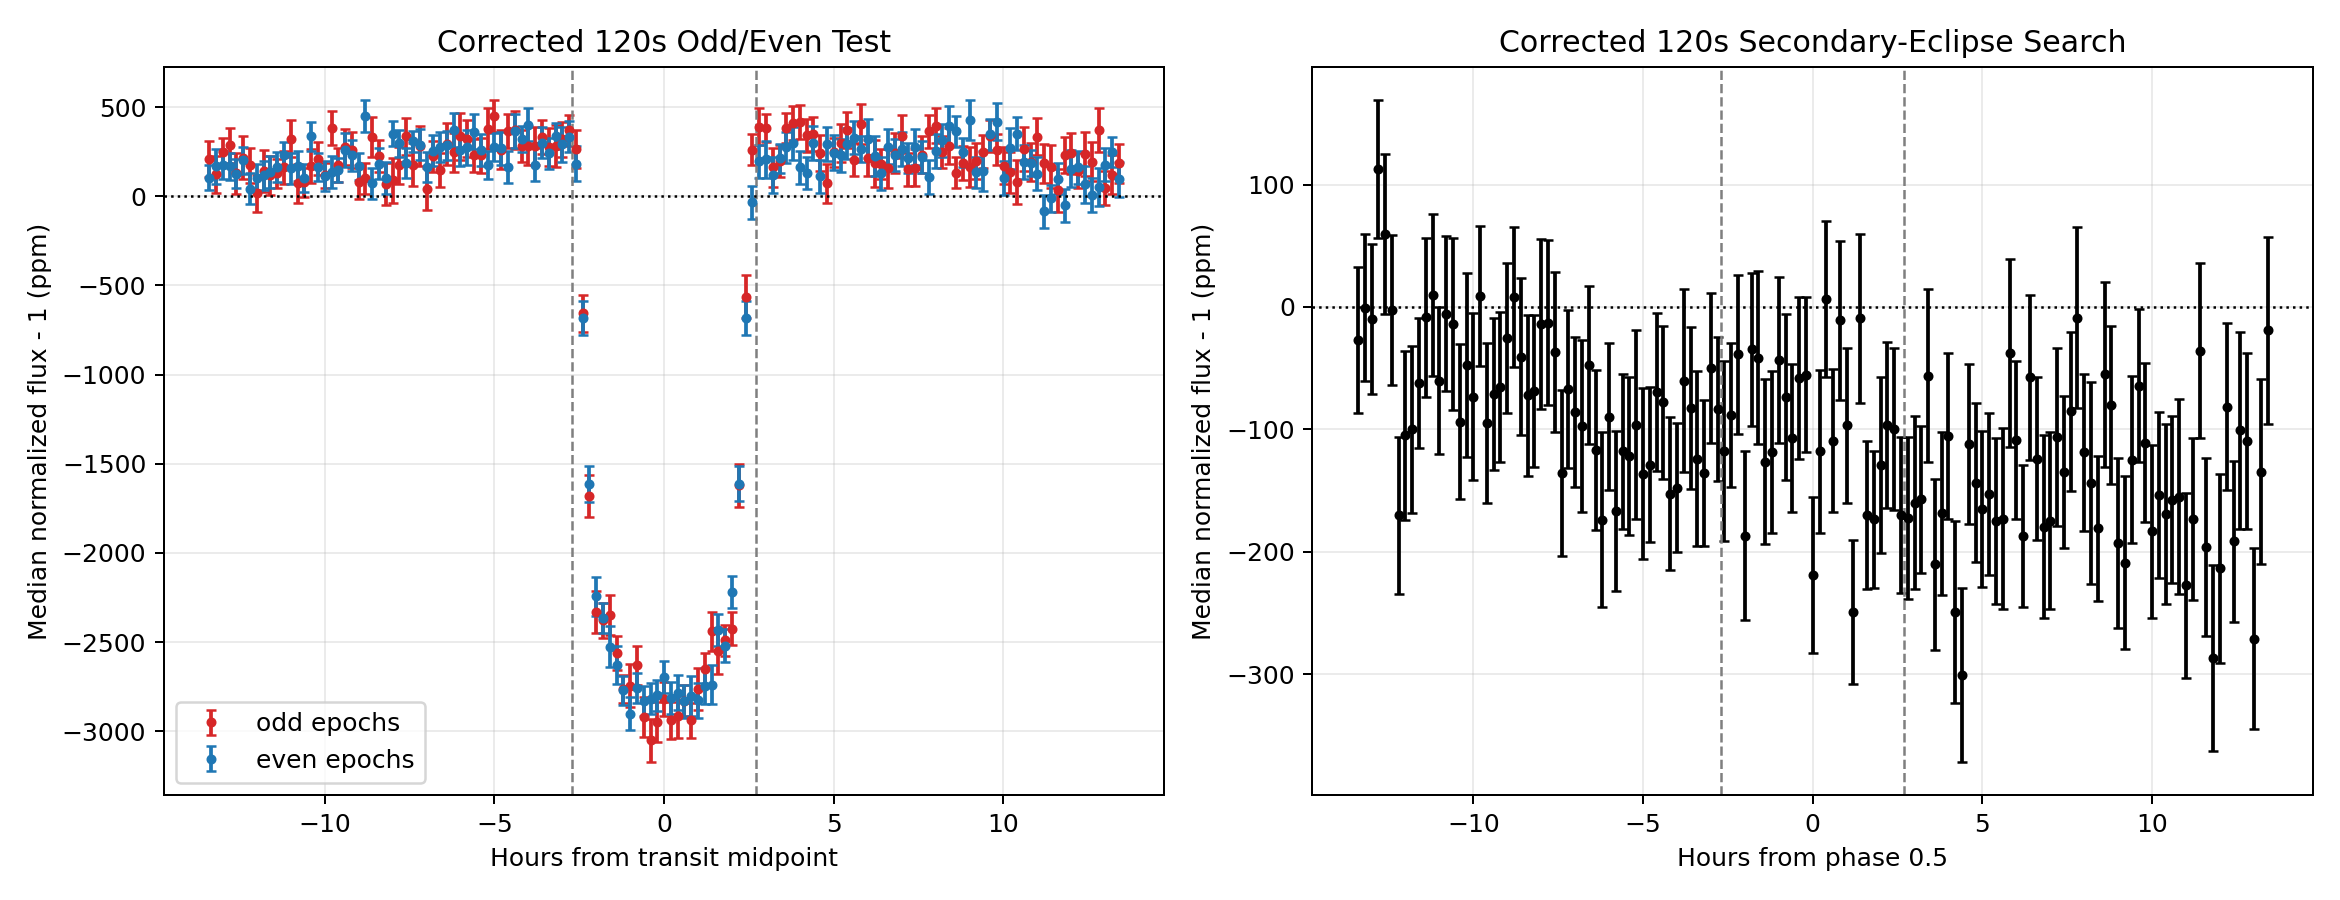
\includegraphics[width=0.95\linewidth]{figures/toi3492_false_positive_120s.png}
\caption{Corrected 120~s odd/even transit-depth comparison (left) and
  secondary-eclipse search near phase~0.5 (right).  These checks reveal no
  significant difference or phase-0.5 eclipse, but do not exclude all
  eclipsing-binary configurations.}
\label{fig:falsepositive}
\end{figure}
The odd/even and phase-0.5 secondary-eclipse diagnostics are shown in
Figure~\ref{fig:falsepositive}.

An additional simultaneous all-phase harmonic regression included terms for
sector offsets and slopes, reflection, beaming, ellipsoidal variations, a
second-harmonic sine, and a secondary eclipse with the transit duration.
Uncertainties were estimated using a 0.5-d
cluster-sandwich covariance over 301 time blocks.  The secondary depth is
$3\pm44$~ppm, giving a conservative $|\hat d|+3\sigma_d$ envelope of 135~ppm.
Here $\hat d$ is the fitted eclipse depth and $\sigma_d$ is its standard error.
The strongest harmonic is a reflection-basis semi-amplitude of
$-144\pm17$~ppm: its sign is opposite to that expected for reflected or
emitted planetary light and remains negative in every sector.  The all-phase analysis is therefore
systematics-limited; no albedo, phase-curve mass, or physical harmonic
detection is reported.  The simpler local phase-0.5 result in
Table~\ref{tab:secondary} is retained as a complementary fixed-window check.
The eclipse box in both analyses is fixed at phase 0.5; no scan over
secondary-eclipse phases allowed by eccentric orbits was performed.  Therefore,
these checks do not
exclude an eccentric eclipsing binary with an occultation at another phase,
and the systematics-limited 135-ppm envelope is not a clean physical upper limit.

\subsection{SPOC Data Validation Products}

The public SPOC Data Validation (DV) products available from
MAST were also parsed.  The local archive contains eight DVT FITS files and eight DVR PDF
reports.  The two multi-sector DV products both identify the official-period
threshold-crossing event (TCE) on the several-thousand-ppm depth scale,
supporting the
corrected 120~s analysis (Table~\ref{tab:spocdv}).  The S1--S96 DV product,
which includes the longest available baseline in the local DV set, reports
$P=9.22240805$~d, depth $=3128.3$~ppm, $a/R_\star=10.248$,
$R_p=15.66\,R_\oplus$, ingress duration 0.559~h, and a multiple-event statistic
(MES) of 99.4 for TCE~1.
The corresponding DVR dashboard rounds these values to
depth $=3128\pm30$~ppm and $R_p=15.7\pm0.7\,R_\oplus$ with a signal-to-noise
ratio (S/N) of 106.

\begin{table}[ht]
\centering
\caption{SPOC DV official-period consistency checks.  Values are parsed from
  local DVT FITS headers except where noted.  The S99 single-sector product
  recovered the same deep signal at the 2$P$ alias.}
\label{tab:spocdv}
\begin{tabular}{lcccc}
\toprule
Product & Relation & Period (d) & Depth (ppm) & MES \\
\midrule
S1--S65  & official $P$ & 9.222417 & 3109.8 & 81.0 \\
S1--S96  & official $P$ & 9.222408 & 3128.3 & 99.4 \\
S37      & official $P$ & 9.222977 & 3043.0 & 42.6 \\
S64      & official $P$ & 9.222730 & 3200.8 & 56.5 \\
S90      & official $P$ & 9.223049 & 3179.8 & 58.7 \\
S100     & official $P$ & 9.221581 & 3028.2 & 48.8 \\
S99      & 2$P$ alias   & 18.444263 & 3111.7 & 44.9 \\
\bottomrule
\end{tabular}
\end{table}

The S1--S96 DVR dashboard reports a joint centroid offset distance of
$2.25\pm2.50$~arcsec, corresponding to $0.90\,\sigma$, and a multi-sector
offset distance of $2.07\pm2.79$~arcsec, corresponding to $0.74\,\sigma$.
Thus the public SPOC DV products are consistent with a source near the target
position, but they do not establish that TIC~81077799 is the source.  They
remain archival diagnostics rather than calibrated PRF localization,
statistical validation, or dynamical confirmation.

\subsection{Statistical Interpretation}

No calibrated false-positive probability is reported.  Odd/even and
secondary-eclipse measurements, a Gaia neighbor census, and archival SPOC
diagnostics do not constitute a population model for the planetary,
eclipsing-binary, hierarchical eclipsing-binary, and background eclipsing-binary
hypotheses.  Normalizing
hand-selected prior weights would produce a number controlled by those
weights rather than by a validated scenario calculation.  The diagnostics
in this section therefore retain their direct observational interpretation:
they do not identify a false-positive source at their present sensitivity, but
they also do not statistically validate or confirm TOI-3492.01.  A validation analysis would require a
calibrated population code, complete scenario likelihoods, a TESS-band
source-localization model, and preferably a high-resolution-imaging contrast
curve \citep{Morton2012,Morton2016,Giacalone2021}.

\subsection{Gaia~DR3 Neighbor Field}

A Gaia~DR3 \citep{Vallenari2023} query within 120~arcsec of the official TOI coordinates
identifies the target as Gaia~DR3~source~5347362071701193344, separated by
only 0.006~arcsec from the TOI coordinate.  The target has a renormalized unit
weight error (RUWE) of 0.985, below the common 1.4 caution threshold and
reassuring for the Gaia single-source astrometric fit.  The Gaia
duplicated-source flag is \texttt{true} and is retained as a caution flag.  A
\texttt{non\_single\_star} value of 0 means that Gaia~DR3 publishes no
non-single-star solution for this source; it does not establish singleness.

For the corrected 3094~ppm transit depth, a fully eclipsed contaminating
source would need to be within $\Delta G = 6.27$~mag of the target, where
$\Delta G=G_{\rm contaminant}-G_\star$.  The
nearest Gaia neighbor is at 7.37~arcsec with $\Delta G = 10.65$, which is
far too faint.  Table~\ref{tab:gaia} summarizes the neighbor census by
search radius.

\begin{table}[ht]
\centering
\caption{Gaia~DR3 neighbor contamination census around TIC~81077799.
  Columns show the cumulative search radius, total neighbor count, the number
  of sources bright enough to mimic the signal as a fully eclipsed
  contaminant or as a 50\% eclipsing binary, and the summed Gaia-band
  flux ratio.}
\label{tab:gaia}
\begin{tabular}{ccccc}
\toprule
Radius & Neighbors & Full-eclipse & 50\% EB & Flux ratio \\
(arcsec) & & mimics & mimics & sum \\
\midrule
21  & 14  & 0 & 0 & 0.00451 \\
42  & 58  & 0 & 0 & 0.01247 \\
60  & 120 & 1 & 0 & 0.02586 \\
120 & 500 & 10 & 7 & 0.24038 \\
\bottomrule
\end{tabular}
\end{table}

No Gaia source inside 42~arcsec is bright enough to mimic the full signal
as a fully eclipsed contaminant.  The source at 56~arcsec could mimic the
depth only if nearly fully eclipsed, and several wider-field sources out to
120~arcsec could mimic it in principle.  Gaia therefore does not identify
an obvious close contaminant but does not replace formal TESS-band source
localization.
The Gaia neighbor field is shown in Figure~\ref{fig:gaia}.

\begin{figure}[ht]
\centering
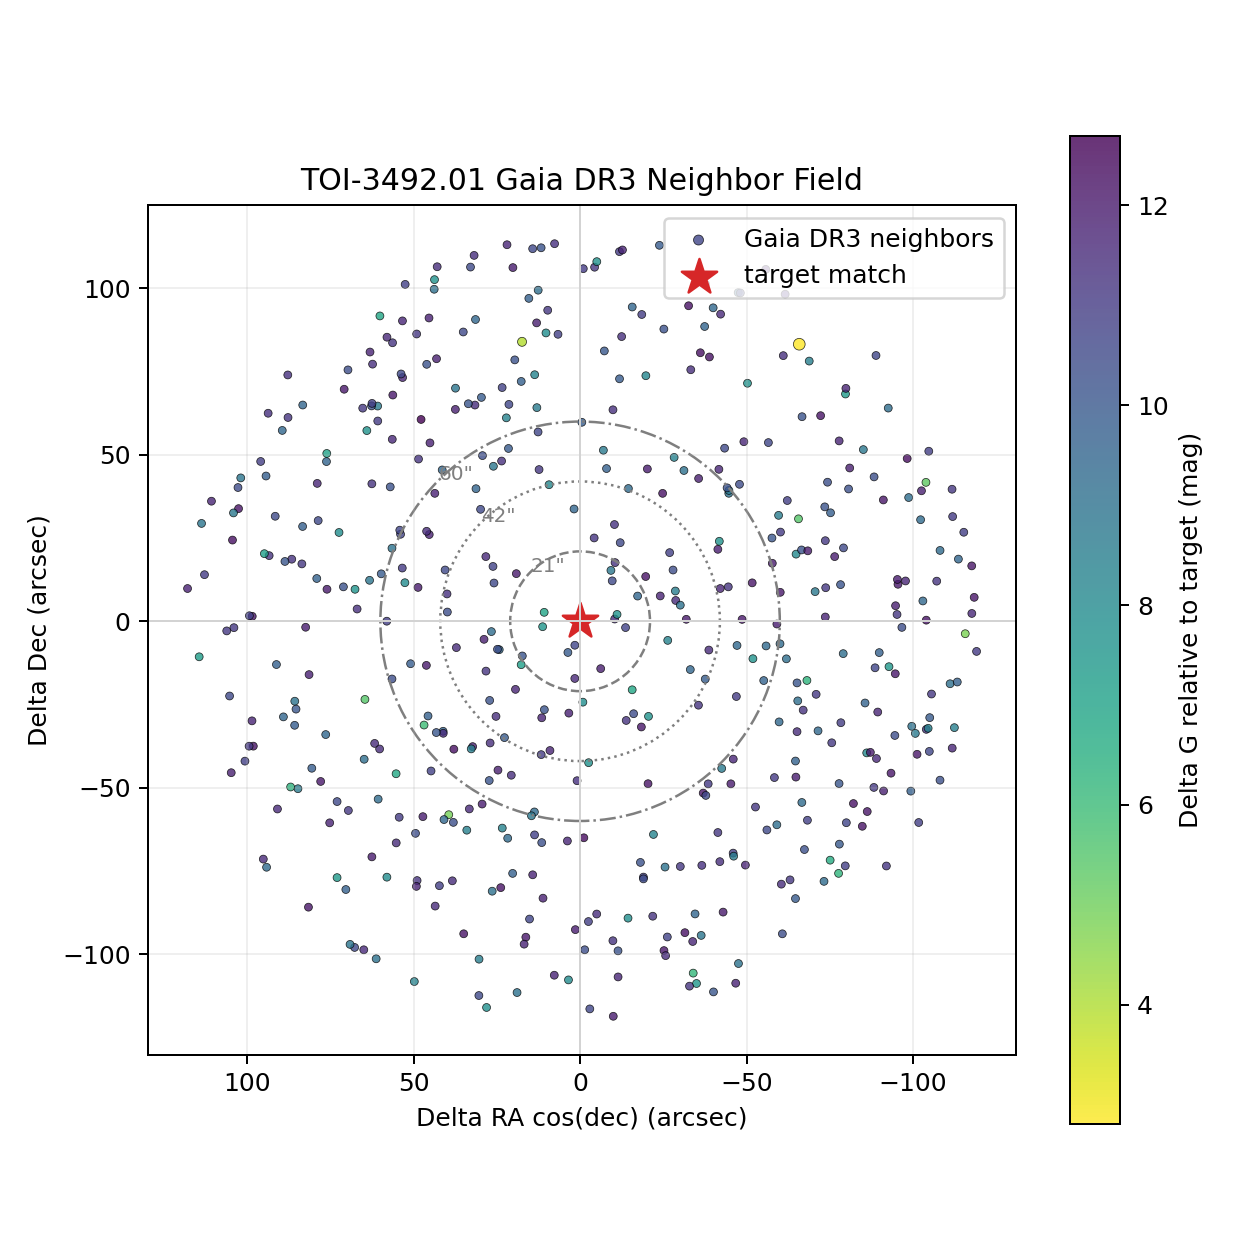
\includegraphics[width=0.85\linewidth]{figures/toi3492_gaia_neighbors.png}
\caption{Gaia~DR3 neighbor field around TIC~81077799.  Circles mark
  approximate 21, 42, and 60~arcsec radii corresponding to the census in
  Table~\ref{tab:gaia}.  Symbol size scales approximately with source
  brightness.  This is a Gaia-band crowding diagnostic, not a formal TESS
  centroid validation.}
\label{fig:gaia}
\end{figure}

\subsection{Dilution Interpretation}

Lightkurve identifies the adopted flux column as SPOC PDCSAP flux, which is
already corrected using the pipeline aperture and crowding terms.  CROWDSAP
is therefore not applied a second time.  The summed Gaia $G$-band neighbor
flux within 42~arcsec is 0.01247 of the target flux, indicating that a
  percent-level crowding uncertainty would not alter the conditional
companion-size scale if the signal originates on TIC~81077799.  This is only a sensitivity
statement because the Gaia $G$ and TESS bandpasses differ and no PRF-weighted aperture
model or high-resolution imaging is available.

\subsection{First-Pass TESS Difference Images}

A first-pass source-localization check was performed using the six 120~s
SPOC target-pixel files (TPFs).  For each sector, the median in-transit pixel
flux was subtracted from the median out-of-transit pixel flux at the
official ephemeris.  The positive difference-image centroid was compared
with the target coordinate projected into the TPF world coordinate system
(WCS).
Table~\ref{tab:diffimages} lists the centroid offsets.

\begin{table}[ht]
\centering
\caption{First-pass TESS difference-image centroid offsets by sector.
  TESS pixels subtend $\approx21$~arcsec.}
\label{tab:diffimages}
\begin{tabular}{cc}
\toprule
Sector & Centroid offset \\
\midrule
37  & 15.0~arcsec ($\approx0.71$~pix) \\
63  & 12.2~arcsec ($\approx0.58$~pix) \\
64  &  1.0~arcsec ($\approx0.05$~pix) \\
90  &  7.2~arcsec ($\approx0.34$~pix) \\
99  & 16.5~arcsec ($\approx0.79$~pix) \\
100 & 22.2~arcsec ($\approx1.06$~pix) \\
\midrule
Median & 13.6~arcsec ($\approx0.65$~pix) \\
\bottomrule
\end{tabular}
\end{table}

All six centroid offsets are within approximately one TESS pixel of the
target coordinate.  This is encouraging and does not point obviously to the
wider Gaia neighbors beyond $\approx$56~arcsec.  However, this is a
first-pass diagnostic only; it was conducted separately from the SPOC~DV
dashboard centroid analysis and does not constitute pixel response function
(PRF) fitting or statistical validation.
We also projected every Gaia source bright enough to mimic a full eclipse into
the frozen TPF WCS and discrete SPOC pipeline masks.  The nearest such source,
at 56.29~arcsec, lies inside every TPF cutout but outside the selected aperture
pixels in all six sectors; each measured difference centroid is closer to the
target than to that source.  This source-specific geometry disfavors the
nearest wider contaminant, but unmodeled PRF wings prevent treating aperture
non-membership as a formal exclusion.  That source has Gaia
\texttt{non\_single\_star}=4 and a $G$-band flux ratio of 0.00431, sufficient
in principle to mimic the event if deeply eclipsed.  Proper-motion propagation,
TESS-band color conversion, aperture throughput, and centroid uncertainties
were not included, so it remains unexcluded.

\begin{figure}[ht]
\centering
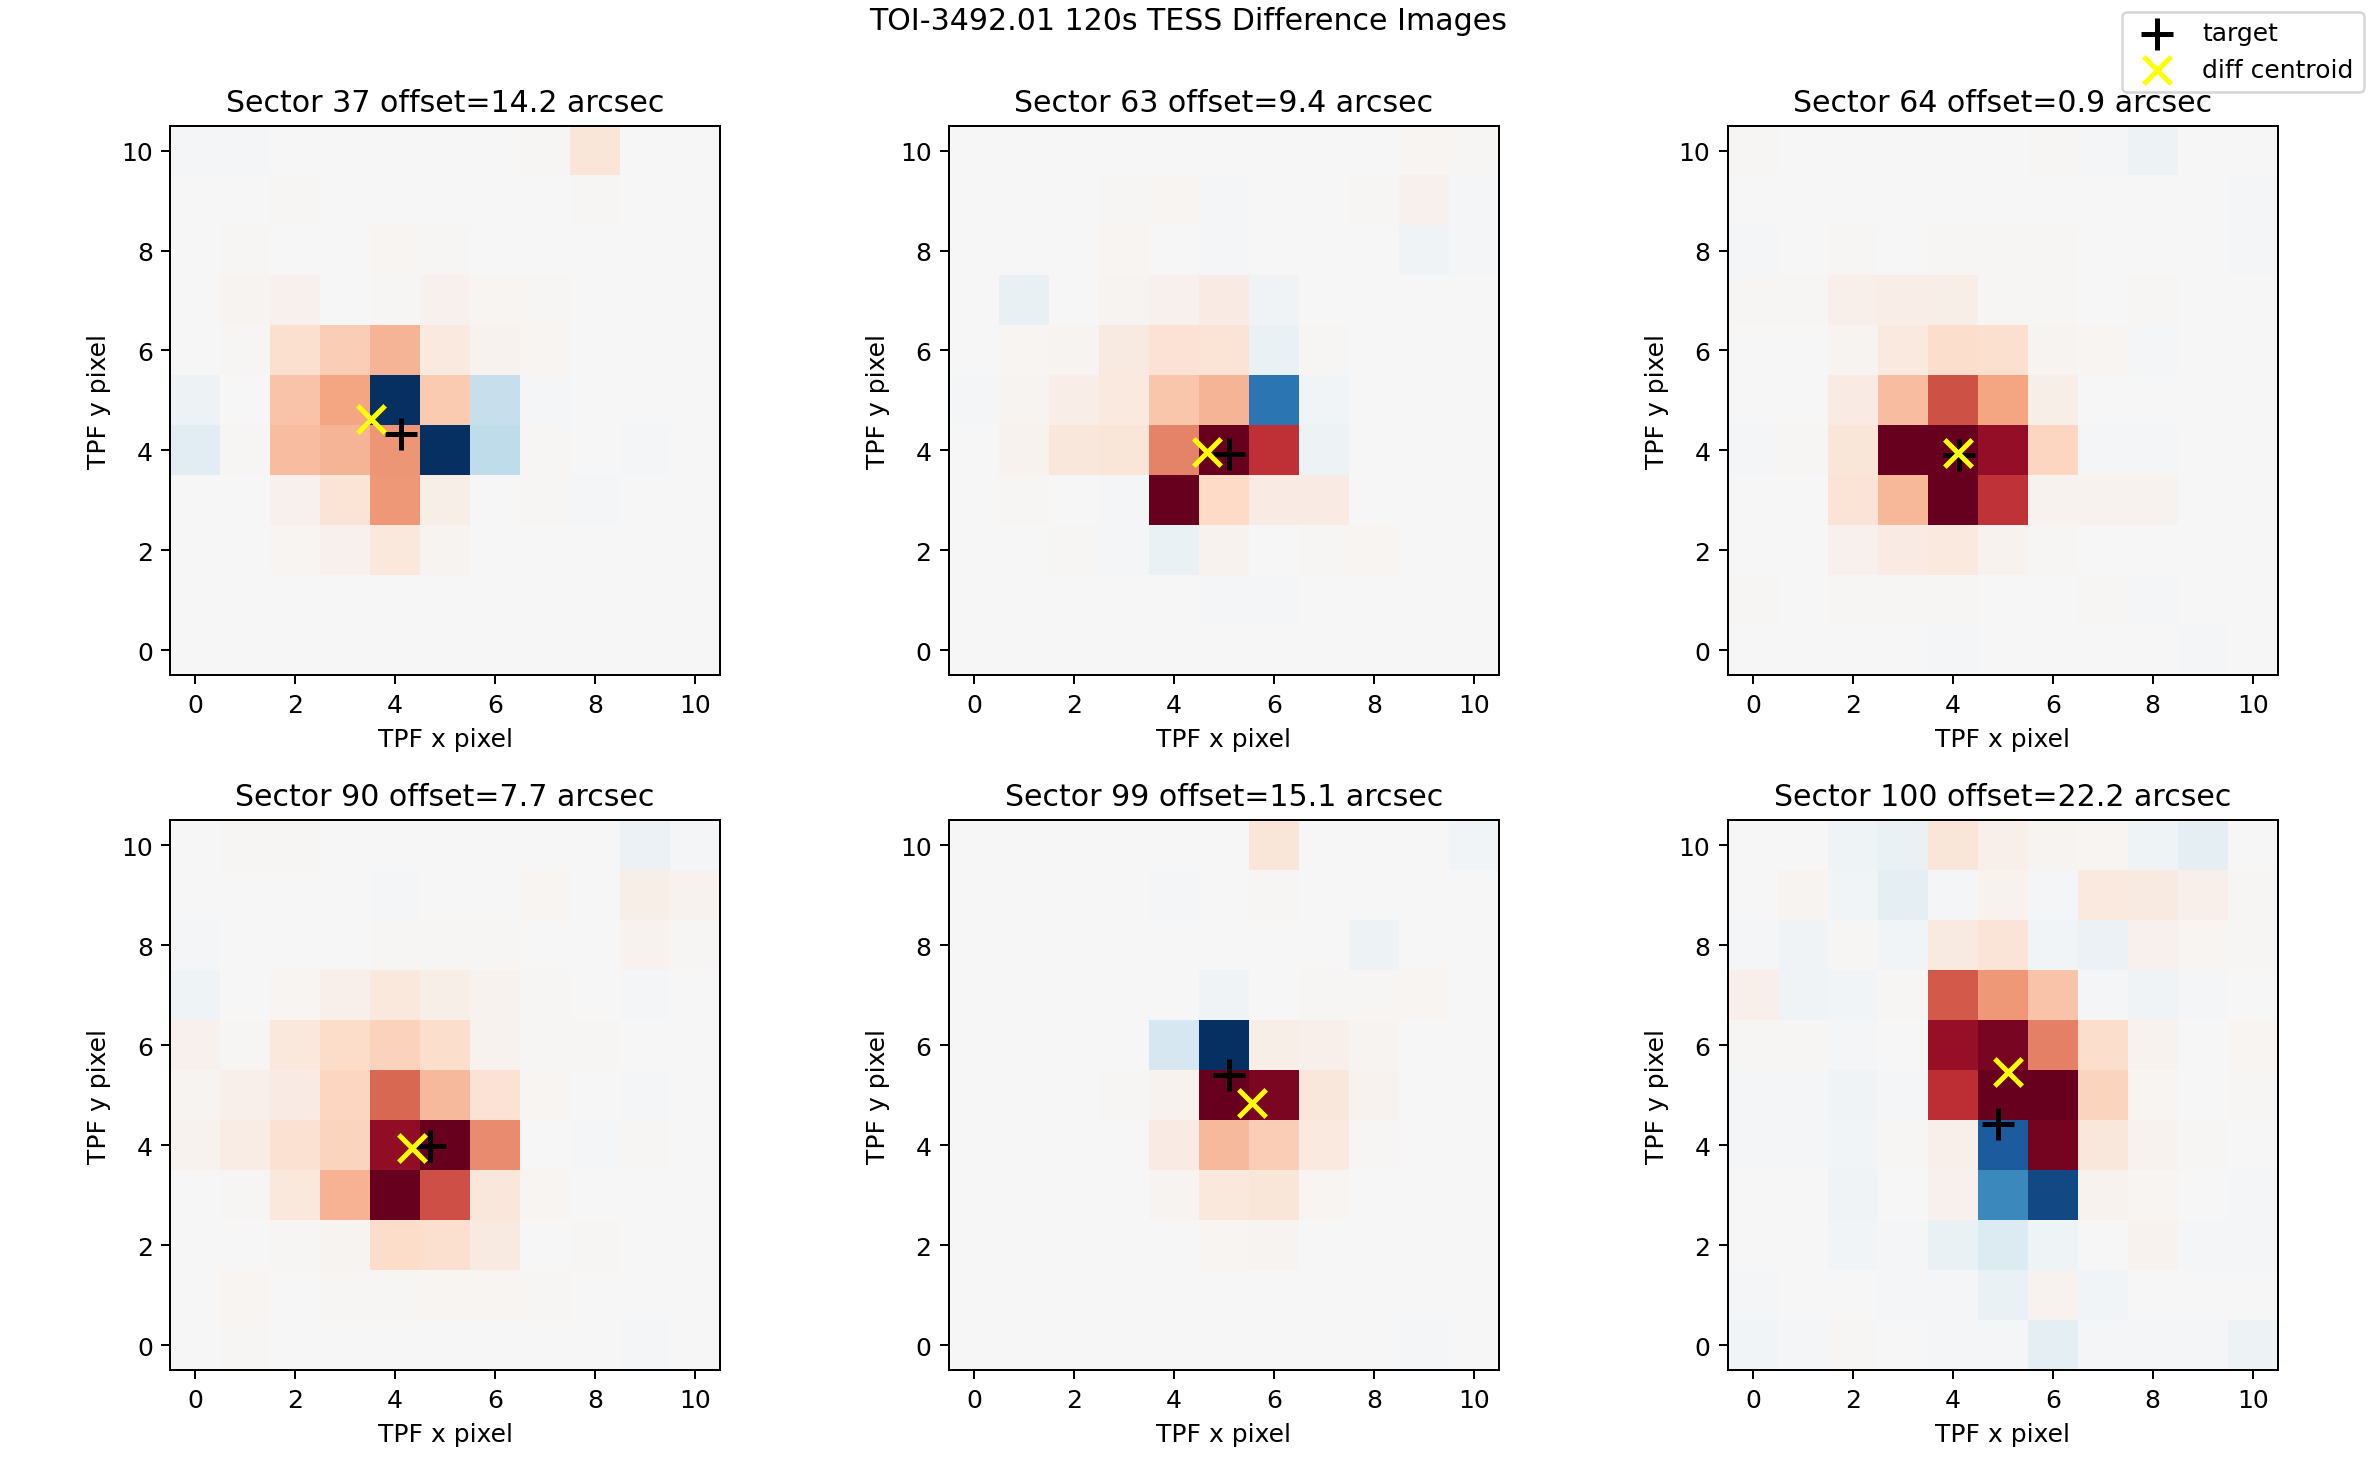
\includegraphics[width=0.95\linewidth]{figures/toi3492_tess_difference_images.png}
\caption{First-pass 120~s TESS difference images for all six sectors.
  Black plus signs mark the target coordinate projected into the TPF~WCS;
  yellow crosses mark the positive difference-image centroid.  All sector
  centroids fall within approximately one TESS pixel ($\approx21$~arcsec)
  of the target.  This analysis is separate from, but based on the same
  observations as, the SPOC~DV dashboard centroid metrics.}
\label{fig:diffimages}
\end{figure}
\FloatBarrier

% -----------------------------------------------------------------------
\section{Discussion}
\label{sec:discussion}
% -----------------------------------------------------------------------

The 120~s phase-folded reference analysis recovers a several-thousand-ppm
event consistent with the official TOI depth scale.  A giant-planet-sized
radius follows only under the joint assumptions that the event is planetary,
originates on TIC~81077799, and the catalog single-star radius is correct.

\paragraph{Vetting and false-positive summary.}
The vetting checks described in Section~\ref{sec:fpvetting} are encouraging but
do not constitute formal validation.  The signal appears in all six 120~s
sectors; fixed-window odd/even and phase-0.5 secondary screens show no
significant feature at their present formal sensitivity; Gaia~DR3 reveals no close bright contaminant inside
42~arcsec; and first-pass TESS difference images place the signal within
approximately one TESS pixel of the target.  These diagnostics do not identify
the sky source or provide a calibrated FPP
(Section~\ref{sec:fpvetting}).  RV confirmation and
calibrated PRF-level source localization remain absent.  No
secondary-eclipse phase scan for eccentric orbits was performed.

\paragraph{Model limitations.}
The phase-folded fit is not a final native-cadence posterior.  Accepted
reduction, mask, window, and polynomial branches produce material sensitivity,
and the original Phase~6 result remains
\texttt{FAIL\_STATIONARITY}.  A later K0 white-plus-jitter numerical-remediation
calculation moved all required starts and passed stationarity in 24/24 branches,
but its maximum weighted residual beta was 1.2936, above the frozen limit of
1.2, giving \texttt{FAIL\_RESIDUAL\_CORRELATION}.  The Stage-3 continuation is
currently protocol-only and has not run a new real-data noise model.  No adopted
geometry, stellar-density discrepancy, or eccentricity measurement follows
from these calculations.  Native-cadence 120~s and 20~s parameter intervals are
omitted, and the converged window comparison is retained only to demonstrate
unpropagated baseline sensitivity.  A passband-integrated
atmosphere/isochrone stellar posterior and reduction-family covariance
propagation are also unavailable.

\paragraph{Interpretation and remaining limitations.}
If the signal is planetary, originates on TIC~81077799, and the catalog
single-star parameters are correct, the descriptive reference scale is
compatible with a short-period giant companion.  Several gaps in the available data prevent a stronger
claim at this stage.  No radial-velocity mass measurement is available,
though the host has TESS magnitude $T_{\rm mag}=8.45$, making RV follow-up
technically feasible.  Independent PRF-level centroid modeling and
high-resolution imaging have not been performed; \citet{LilloBox2024}
found that approximately 7\% of TESS candidates have close companions
unresolved by Gaia~DR3.  The Gaia~DR3 contamination estimates use
$G$-band flux ratios as a proxy for TESS-band dilution rather than a
full TESS-band aperture-contamination model.  As discussed in
Section~\ref{sec:stellar}, none of APOGEE, LAMOST, GALAH, or RAVE has a
match within 5~arcsec, so the critical $\log g$, $T_{\rm eff}$, and
$[\mathrm{Fe}/\mathrm{H}]$ values cannot all be cross-validated without new
observations: $\log g$ and $T_{\rm eff}$ require independent measurements,
while $[\mathrm{Fe}/\mathrm{H}]$ has not yet been measured.  The 20~s products
in Sectors~90, 99, and~100 are retained only as same-pixel cadence diagnostics.

The current work therefore supports a conservative interpretation:
TOI-3492.01 is a persistent transit-like candidate with an unresolved source;
no statistical validation or dynamical confirmation is claimed.  It
should not be used for planet-population interpretation without the
follow-up observations described above.

% -----------------------------------------------------------------------
\section{Summary and Conclusions}
% -----------------------------------------------------------------------

Public TESS photometry of TOI-3492.01 (TIC~81077799) was independently
analyzed, yielding the following:

\begin{enumerate}
  \item TIC~81077799 is an evolved, low-density subgiant-like star
    ($R_\star = 2.5926\pm0.1094\,R_\odot$), despite the TIC
    \texttt{lumclass=DWARF} classification.
  \item A targeted 120~s BLS analysis recovers a periodic signal near the
    official TOI period; it does not independently establish
    the quoted ephemeris precision.
  \item A circular fit to phase-folded, binned photometry provides a
    descriptive reference only.  Its parameter intervals are not adopted as
    native-cadence measurements.  A giant-planet-sized physical scale is
    conditional on a planetary event originating on TIC~81077799 and on the
    catalog single-star parameters.
  \item All six 120~s sectors independently show a deep transit-like signal,
    demonstrating persistence, but their formal depths are heterogeneous
    ($\chi^2=29.85$ for 5 degrees of freedom).
  \item Odd/even and fixed phase-0.5 secondary checks are inconclusive
    screening tests.  SPOC~DV, Gaia~DR3, source-specific aperture, and
    first-pass difference-image checks do not provide calibrated source
    localization.  An all-phase regression is systematics-limited.
  \item No calibrated population FPP is reported; the available checks do
    not statistically validate or confirm the candidate.
  \item Native-cadence fits fail the required convergence/noise-model gates;
    their parameter intervals are omitted.  No stellar-density discrepancy or
    eccentricity measurement is claimed.
  \item A converged fit-window sensitivity comparison shifts $R_p/R_\star$ by
    1.95 reference-posterior half-widths.  The descriptive reference intervals
    do not include this window-choice systematic.
\end{enumerate}

TOI-3492.01 therefore remains an unvalidated and unconfirmed transit-like
candidate with an unresolved source.  The principal next steps are calibrated
PRF-level localization, high-resolution imaging, independent spectroscopy,
and epoch radial velocities.  A dynamical mass or confirmation claim requires
new target-specific observations and separate passing analysis gates.



% -----------------------------------------------------------------------
\section*{Acknowledgements}
% -----------------------------------------------------------------------

This research made use of \texttt{lightkurve}, a Python package for Kepler
and TESS data analysis \citep{Lightkurve2018}, and of data collected by the
TESS mission, which are publicly available from the Mikulski Archive for
Space Telescopes (MAST).  Funding for the TESS mission is provided by NASA's
Science Mission Directorate.  This work has made use of data from the
European Space Agency (ESA) mission \textit{Gaia}
\citep{Vallenari2023}, processed by the \textit{Gaia} Data Processing and
Analysis Consortium (DPAC).


% -----------------------------------------------------------------------
\section*{Data Availability}
% -----------------------------------------------------------------------

The working reproducibility materials contain the corrected 120~s reference
light curve, diagnostic posterior chains, machine-readable transit outputs,
analysis scripts, dependency specification, and SHA-256 provenance records.
Original SPOC light-curve and target-pixel products remain publicly available
from MAST.  A final release package and DOI are deferred until the scientific
claim audit and manuscript are frozen.

% -----------------------------------------------------------------------
\bibliographystyle{plainnat}
\bibliography{references}
% -----------------------------------------------------------------------

\end{document}
